
%(BEGIN_QUESTION)
% Copyright 2010, Tony R. Kuphaldt, released under the Creative Commons Attribution License (v 1.0)
% This means you may do almost anything with this work of mine, so long as you give me proper credit

An Automation Direct model C0-08TD2 ``sourcing'' DC output PLC module uses the following internal circuitry to switch DC power to a load:

$$\includegraphics[width=15.5cm]{i03665x01.eps}$$

Suppose the microprocessor is sending a ``high'' (1) signal to the switching circuitry, but the DC load refuses to energize.  Using your DC voltmeter, you measure 24.7 volts DC between the ``+V'' and ``Com'' terminals, and 0 volts DC between the ``Out'' and ``Com'' terminals.

\vskip 10pt

Identify the likelihood of each specified fault for this circuit.  Consider each fault one at a time (i.e. no coincidental faults), determining whether or not each fault could independently account for {\it all} measurements and symptoms in this circuit.

% No blank lines allowed between lines of an \halign structure!
% I use comments (%) instead, so that TeX doesn't choke.

$$\vbox{\offinterlineskip
\halign{\strut
\vrule \quad\hfil # \ \hfil & 
\vrule \quad\hfil # \ \hfil & 
\vrule \quad\hfil # \ \hfil \vrule \cr
\noalign{\hrule}
%
% First row
{\bf Fault} & {\bf Possible} & {\bf Impossible} \cr
%
\noalign{\hrule}
%
% Another row
Diode $D_1$ failed shorted &  &  \cr
%
\noalign{\hrule}
%
% Another row
Diode $D_2$ failed open &  &  \cr
%
\noalign{\hrule}
%
% Another row
Diode $D_3$ failed open &  &  \cr
%
\noalign{\hrule}
%
% Another row
Diode $D_4$ failed open &  &  \cr
%
\noalign{\hrule}
%
% Another row
Transistor $Q_1$ failed open &  &  \cr
%
\noalign{\hrule}
%
% Another row
Transistor $Q_2$ failed open &  &  \cr
%
\noalign{\hrule}
%
% Another row
Transistor $Q_3$ failed shorted &  &  \cr
%
\noalign{\hrule}
%
% Another row
Capacitor $C_1$ failed open &  &  \cr
%
\noalign{\hrule}
%
% Another row
Resistor $R_1$ failed shorted &  &  \cr
%
\noalign{\hrule}
%
% Another row
Resistor $R_2$ failed shorted &  &  \cr
%
\noalign{\hrule}
%
% Another row
Resistor $R_3$ failed open &  &  \cr
%
\noalign{\hrule}
%
% Another row
Resistor $R_4$ failed open &  &  \cr
%
\noalign{\hrule}
%
% Another row
Resistor $R_5$ failed shorted &  &  \cr
%
\noalign{\hrule}
%
% Another row
Resistor $R_6$ failed open &  &  \cr
%
\noalign{\hrule}
} % End of \halign 
}$$ % End of \vbox

Finally, identify the {\it next} diagnostic test or measurement you would make on this system.  Explain how the result(s) of this next test or measurement help further identify the location and/or nature of the fault.

\vfil 

\underbar{file i03665}
\eject
%(END_QUESTION)





%(BEGIN_ANSWER)

% No blank lines allowed between lines of an \halign structure!
% I use comments (%) instead, so that TeX doesn't choke.

$$\vbox{\offinterlineskip
\halign{\strut
\vrule \quad\hfil # \ \hfil & 
\vrule \quad\hfil # \ \hfil & 
\vrule \quad\hfil # \ \hfil \vrule \cr
\noalign{\hrule}
%
% First row
{\bf Fault} & {\bf Possible} & {\bf Impossible} \cr
%
\noalign{\hrule}
%
% Another row
Diode $D_1$ failed shorted &  & $\surd$ \cr
%
\noalign{\hrule}
%
% Another row
Diode $D_2$ failed open & $\surd$ &  \cr
%
\noalign{\hrule}
%
% Another row
Diode $D_3$ failed open & $\surd$ &  \cr
%
\noalign{\hrule}
%
% Another row
Diode $D_4$ failed open &  & $\surd$ \cr
%
\noalign{\hrule}
%
% Another row
Transistor $Q_1$ failed open & $\surd$ &  \cr
%
\noalign{\hrule}
%
% Another row
Transistor $Q_2$ failed open & $\surd$ &  \cr
%
\noalign{\hrule}
%
% Another row
Transistor $Q_3$ failed shorted &  & $\surd$ \cr
%
\noalign{\hrule}
%
% Another row
Capacitor $C_1$ failed open &  & $\surd$ \cr
%
\noalign{\hrule}
%
% Another row
Resistor $R_1$ failed shorted &  & $\surd$ \cr
%
\noalign{\hrule}
%
% Another row
Resistor $R_2$ failed shorted &  & $\surd$ \cr
%
\noalign{\hrule}
%
% Another row
Resistor $R_3$ failed open & $\surd$ &  \cr
%
\noalign{\hrule}
%
% Another row
Resistor $R_4$ failed open &  & $\surd$ \cr
%
\noalign{\hrule}
%
% Another row
Resistor $R_5$ failed shorted & $\surd$ &  \cr
%
\noalign{\hrule}
%
% Another row
Resistor $R_6$ failed open & $\surd$ &  \cr
%
\noalign{\hrule}
} % End of \halign 
}$$ % End of \vbox


%(END_ANSWER)





%(BEGIN_NOTES)


%INDEX% Troubleshooting review: electric circuits

%(END_NOTES)

